
%
%  $Description: Author guidelines and sample document in LaTeX 2.09$ 
%
%  $Author: ienne $
%  $Date: 1995/09/15 15:20:59 $
%  $Revision: 1.4 $
%

\documentclass[times, 10pt,twocolumn]{article} 
\usepackage{latex8}
\usepackage{times}
\usepackage{graphicx}
\usepackage{subcaption}


%\documentstyle[times,art10,twocolumn,latex8]{article}

%------------------------------------------------------------------------- 
% take the % away on next line to produce the final camera-ready version 
\pagestyle{empty}

%------------------------------------------------------------------------- 
\begin{document}

% \title{Epidemics Graph Neural Network Node Classification}
\title{Epidemics Graph Neural Network Node Classification and Link Prediction}

\author{Jaykumar Patel\\
patel.jay4802@utexas.edu\\
% For a paper whose authors are all at the same institution, 
% omit the following lines up until the closing ``}''.
% Additional authors and addresses can be added with ``\and'', 
% just like the second author.
\and
Afnan Mir\\
afnanmir@utexas.edu\\
}

\maketitle
\thispagestyle{empty}

\begin{abstract}
The COVID-19 pandemic showed that contact tracing helped mitigate the spread of the virus. However, manual contact tracing is slow and can be inaccurate. Thus, this project aims to automate contact tracing by utilizing Graph Neural Networks (GNNs). Our preliminary work on network analysis showed that the contact network is a mix of an exponential and scale-free network. Also, our simulation showed that during the first 12 hours, the infection does not spread much, but then it starts spreading steadily. 
\end{abstract}


%------------------------------------------------------------------------- 
\Section{Introduction and Motivation}

When COVID-19 first appeared, manual tracing was deployed to mitigate the initial outbreak. Contact tracing is the process of tracking how the virus spreads by identifying people who may have come in contact with an infected person, and then asking them to isolate and get tested.

However, the pandemic revealed that the COVID-19 virus spread faster than manual contact tracing \cite{flaxman2020estimating}. Thus, this project's objective is to automate contact tracing by incorporating machine learning using GNNs to hopefully increase the mitigation of the spread of COVID-19 when compared to manual contact tracing.

% - What is the big picture? What is the main objective of this project?
% - Why is this project interesting?

%------------------------------------------------------------------------- 

\Section{Previous Work}
% Methods for predicting the spread of COVID-19 include mathematical models, traditional ML models, and graph-based ML models. 

% One example of a mathematical model is the SEIRD model, which attempts to predict the change in Susceptible, Exposed, Infected, Recovered, and Deceased people over time through use of differential equations. This model is used to simulate the spread of the virus over time \cite{SEIRD-LSTM}.
% % (https://www.frontiersin.org/articles/10.3389/fpubh.2021.727274/full)
% SIR is simpler version of the SIERD model that attempts to perform the same task \cite{SIR}.
% % https://www.medrxiv.org/content/10.1101/2020.05.15.20103077v2

% Traditional ML models have also been used to predict the spread of COVID-19. For example, Long Short-Term Memory (LSTM) models have been used to predict the number of cases over time \cite{SEIRD-LSTM}. 
% % https://www.frontiersin.org/articles/10.3389/fpubh.2021.727274/full
% Another approach utilizes a hybrid of SIRD and LSTM to account for time dependent parameters of the SIRD model \cite{SIRD-LSTM-hybrid}.
% % https://www.nature.com/articles/s41598-022-06992-0

% Furthermore, graph-based ML models, such as GNNs, have been used on mobility data to predict the number of cases and hospitalizations \cite{positivity-hospitalization-GNN}.
% % https://www.ncbi.nlm.nih.gov/pmc/articles/PMC10066232/#:~:text=Message%20passing%20instances%20of%20GNNs,as%20well%20as%20hospitalization%20rates.
% GNNs can also be used for link prediction, which is useful for contact tracing \cite{contact-tracing-GNN}. 
% % https://proceedings.neurips.cc/paper_files/paper/2018/file/53f0d7c537d99b3824f0f99d62ea2428-Paper.pdf

% Methods for predicting the spread of COVID-19 include mathematical models, traditional ML models, and graph-based ML models. 

Mathematical models, classical ML models, and graph-based ML models have been used to predict virus spread. 

The SEIRD model is a mathematical model that predicts the change in Susceptible, Exposed, Infected, Recovered, and Deceased people over time by using differential equations. \cite{SEIRD-LSTM}. SIR is simpler version of the SIERD model \cite{SIR}.

The LSTM is an ML model that has been used to predict the number of cases over time \cite{SEIRD-LSTM}. A hybrid of SIRD and LSTM helps account for time dependent parameters of the SIRD model \cite{SIRD-LSTM-hybrid}. Also, GNNs, which are graph-based ML models, have been used on mobility data to predict virus spread and for link prediction for contact tracing \cite{positivity-hospitalization-GNN}\cite{contact-tracing-GNN}.
% The LSTM is a ML model that has also been used to predict the number of cases over time \cite{SEIRD-LSTM}. Another approach uses a hybrid of SIRD and LSTM to account for time dependent parameters of the SIRD model \cite{SIRD-LSTM-hybrid}.
% Other approaches include the Long Short-Term Memory (LSTM) model \cite{SEIRD-LSTM} and a hybrid of SIRD and LSTM \cite{SIRD-LSTM-hybrid}.

% Also, GNNs, which are graph-based ML models, have been used on mobility data to predict the number of cases and hospitalizations \cite{positivity-hospitalization-GNN}. GNNs have also been used for link prediction, which is useful for contact tracing \cite{contact-tracing-GNN}. 

% Also, GNNs, which are graph-based ML models, have been used on mobility data to predict virus spread \cite{positivity-hospitalization-GNN}. GNNs have also been used for link prediction for contact tracing \cite{contact-tracing-GNN}. 
% Also, GNNs, which are graph-based ML models, have been used on mobility data to predict virus spread \cite{positivity-hospitalization-GNN} for link prediction for contact tracing \cite{contact-tracing-GNN}. 


% Feature Based Approach:
%     - Multivariate Logistic Regression to predict infectious risk
%     - Might not be an actual study, just a proposal
% https://www.ncbi.nlm.nih.gov/pmc/articles/PMC8570232/#Sec2title


% https://www.frontiersin.org/articles/10.3389/fpubh.2021.727274/full
% Uses 2 approaches:
% SEIRD - Susceptible, Exposed, Infectious, Recovered, Deceased
%     - simulating the spread of the virus over time
%     - Simulation Approach
% LSTM
%     - To predict the number of cases over time by training the NN over a subset of time
%     - ML Approach

% Previously used methods for predicting infections include mathemical models and ML models.
% One example of a mathemical model is the SEIRD model, which attempts to predict the change in Susceptible, Exposed, Infected, Recovered, and Deceased people over time through the use of differential equations. This model is used to simulate the spread of the virus over time. 

% https://www.ncbi.nlm.nih.gov/pmc/articles/PMC10066232/#:~:text=Message%20passing%20instances%20of%20GNNs,as%20well%20as%20hospitalization%20rates.
%     - utilizes GNNs on mobility data to predict number of cases and hospitalizations


% https://www.nature.com/articles/s41598-021-97037-5
%     - Combined mathemical and ML models
%     - Specifically uses LSTM to predict number of cases over time
%     - Uses Markov Model to reduce prediction error of the LSTM

% https://www.nature.com/articles/s41598-022-06992-0
%     - Combines LSTM and SIRD
%     - Uses LSTM to solve for the time dependent parameters of the SIRD model
%     - Uses LSTM to predict the number of cases over time









\Section{Approach}
\subsection{Network Generation and Analysis}
% We used the foursquare dataset to build a contact graph of Austin, Texas \cite{DVN/PFLAH4_2020}. Each entry contains data such as a device ID, a location ID, UTC date and hour, and a dwell time, which all tell us when a person visited a location and for how much time. Given this data, we generated a contact graph for people in Austin.

We used the foursquare dataset to build a contact graph of Austin, TX \cite{DVN/PFLAH4_2020}. Each entry contains a device ID, a location ID, UTC date and hour, and a dwell time, which tell us when and how long a person visited a location. Given this data, we generated a contact graph of Austin.

% We used data only from July 1st, 2020 to generate a sample network. Our nodes were all the unique device IDs in the dataset, which correspond to people. For our edges, we used the following logic: we ignored entries with a dwell time less than 60 minutes, as we assumed this not enough time to make significant contact with others. Then, we used the UTC date and hour with the dwell time to determine the arrival and departure time interval for each entry. We then compared every entry with every other entry. If the entries' locations were the same and if intervals overlapped by at least 60 minutes, we considered this as a contact between the two people and added an edge between them. Figure \ref{fig:toy_label} shows an example of a sample contact network generation. 

Firstly, we used data from July 1st, 2020 to July 5th, 2020 to create a sample contact network. Our nodes were all the unique device IDs in the dataset, which correspond to people. For our edges, we used the following logic: we ignored entries with a dwell time less than 60 minutes, as we assumed this not enough time to make significant contact with others. Then, we used the UTC date and hour with the dwell time to determine the arrival and departure time interval for each entry. We then compared every entry with every other entry. If the entries' locations were the same and if intervals overlapped by at least 60 minutes, we considered this as a contact between the two people and added an edge between them. We will call this the 5-Day Contact Network. This network captures the meaningful contacts that occurred from July 1st, 2020 to July 5th, 2020. Figure \ref{fig:toy_label} shows an example of a sample contact network generation. 

\begin{figure}
    \centering
    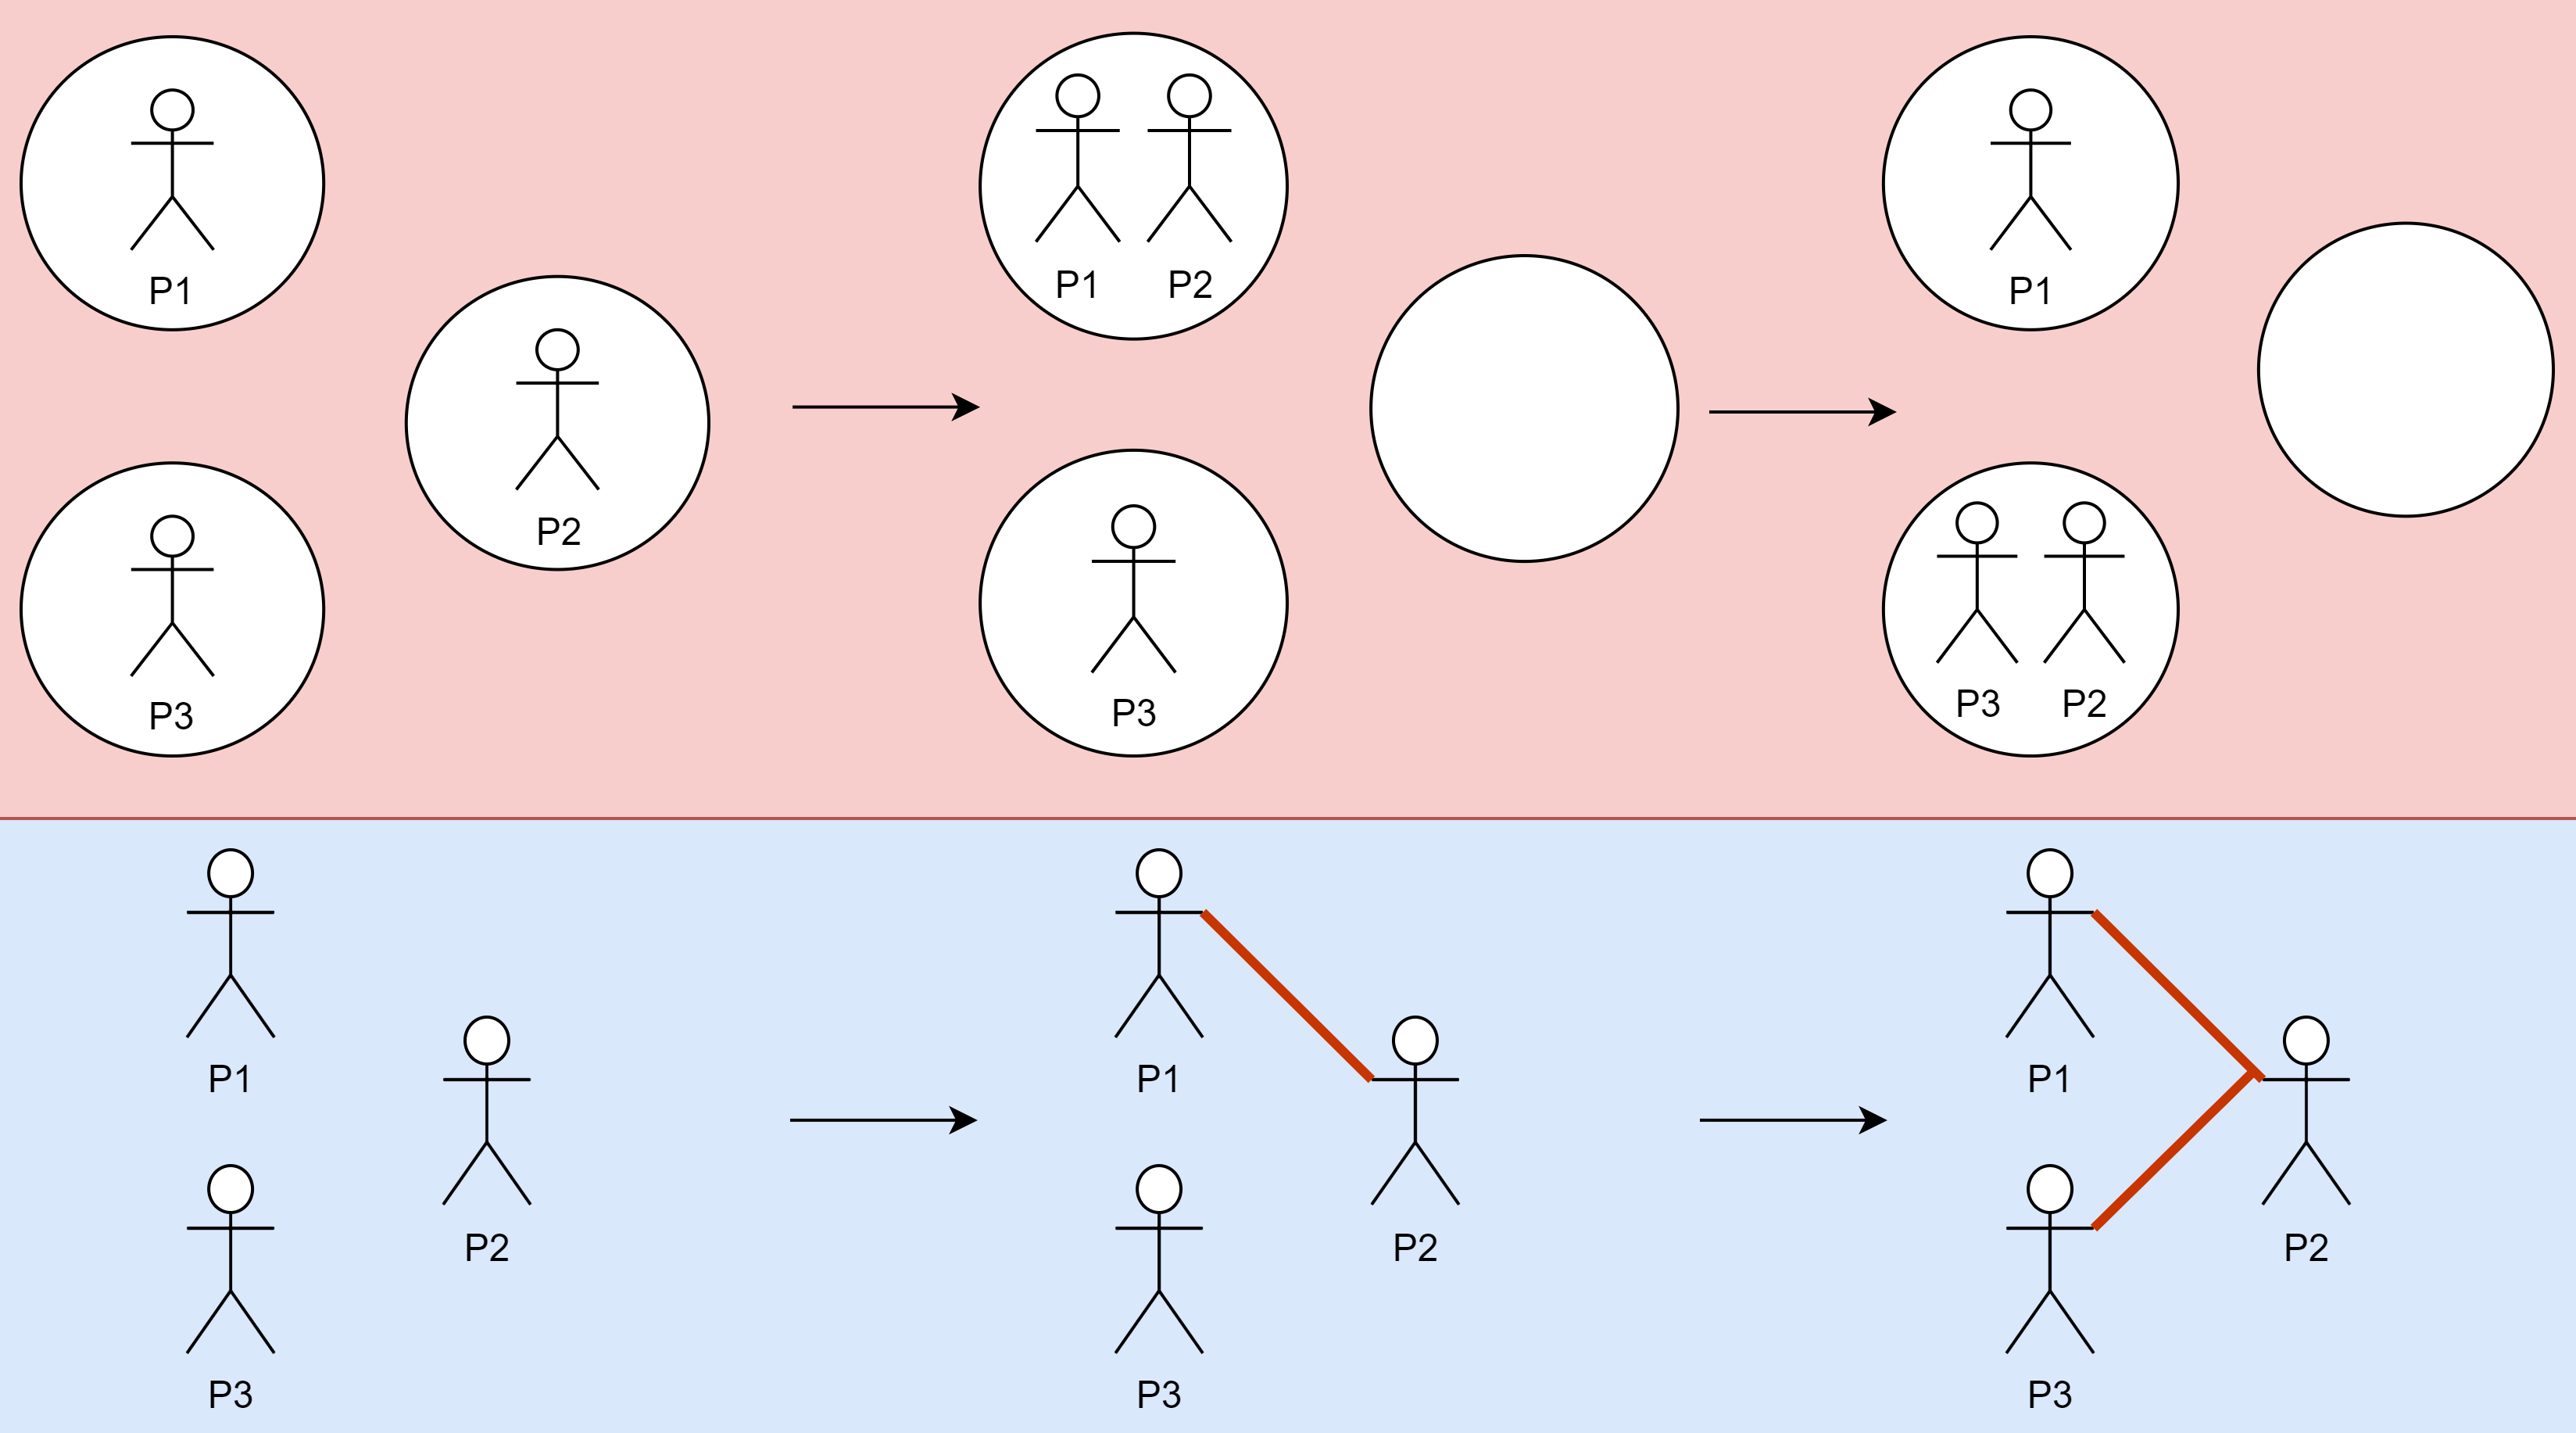
\includegraphics[width=0.30\textwidth]{imgs/Network_Toy.png}
    \caption{Example of contact network generation}
    \label{fig:toy_label}
\end{figure}

Then we also created a set of 62 contact networks, one for each day from July 1st, 2020 to August 31st, 2020. We used the same logic as before to create these individual contact networks. We will call this set of networks the Temporal Contact Networks. Each day's network captures the meaningful contacts that occurred for that day. The Temporal Contact Networks allow us to analyze the contact network over time at daily increments. Particularly, we analyzed how the following metrics change over time:
\begin{itemize}
    \item Clustering Coefficient
    \item Average Node Degree
\end{itemize}

We also created a Susceptible-Infected-Recovered simulation using the Temporal Contact Networks. We ran the simulation from July 1st, 2020 to August 31st, 2020. Here are the parameters and assumptions that were made for the simulation:
\begin{itemize}
    \item Contact between people that is less than 60 minutes is not considered significant enough to spread the virus.
    \item If a susceptible person came into contact with an infected person for at least one hour, then they get infected with a probability of 0.30. This is called the infection rate (IR).
    \item The IR is constant throughout the simulation.
    \item An infected person will recover after seven days. This is called the recovery period (RP).
    \item The RP is constant throughout the simulation.
    \item A person can only be infected if they were previously susceptible, and a person can only be recovered if they were previously infected.
    \item Initially, 20\% of the people, chosen at random, are infected. The rest are susceptible.
    \item Only infected people can infect others.
\end{itemize}

\subsection{Machine Learning}

% there was an overlap of at least 60 minutes in their dwelling times, we considered this as a contact between the two people. We then added an edge between the two people in our graph.

% Separately, we also created a sample Susceptible-Infected (SI) simulation using data from July 1st, 2020. We did not include a recovery/death or incubation period in this model mainly because we only performed the simulation over one day. For the simulation, we did the following: at hour 0, we randomly infected 20\% of the nodes in the graph. Then we looked at all contacts between people for hour 1, and if an infected person came into contact with a susceptible person, we created an edge between them and infected the susceptible person with a probability of 1. We repeated the previous step for the remaining 22 hours of the day.

After generating and analyzing the 5-Day Contact Network, Temporal Contact Networks, and performing the SIR simulation, we moved towards leveraging graph learning techniques to perfom link prediction, which is the fundamental task behind automating contact tracing. For this milestone, we focused on performing link prediction on a static graph. In order to have enough data to train and evaluate our model(s), we generated a contact network for the first five days of July. We used the same technique described in building our July 1st contact network to build the 5 day contact network; so the nodes are people who have a dwell time of at least 60 minutes at one location, and edges represent people who have come into contact with each other in the 5 day period. 

Our first goal was to create a baseline link prediction model. We used the node2vec algorithm to generate node embeddings for each node in the graph \cite{grover2016node2vec}. We then had to generate our dataset of edges. In order to perform link prediction, we need the set of positive edges, which are the edges present in the network, and we need a set of negative edges, which are the edges not present the network. This allows us to boil down the link prediction to a binary classification problem. Given our network, we created a set of negative edges that was equal in size to the set of positive edges to ensure balanced training. Using the node2vec embeddings and the set of positive and negative edges, we trained a GraphSAGE model to perform link prediction on the static 5 day graph \cite{hamilton2018inductive}.

After creating the baseline model, we searched for ways to improve the model's performance on the graph. This would include performing feature engineering techniques to add dimensions to our node embeddings and exploring the use of other GNN architectures such as GCN and/or GAT \cite{kipf2017semisupervised} \cite{veličković2018graph}. We hoped to be able to finetune the model and improve its performance to the point we could use it to perform link prediction on the Temporal Contact Networks. 

Here are the additional featues the generated for every node (person) in the graph:
\begin{itemize}
    \item Average location travelled to per day
    \item Average distance travelled per day
    \item Gender
    \item SAG Score
    \item Age
\end{itemize}
% Then for each hour from 1 to 23, we looked at all contacts between people, and if an infected person came into contact with a susceptible person, we infected the susceptible person with a probability of 1.0. We did this for 24 hours.

% Next, with each time step (1 hour), we looked at all the neighbors of each infected node and infected them with a probability of 1.0, so we assumed any contact led to an infection. We did this for 24 hours.


\Section{Experimental Setup and Results}

% \begin{figure}
%     \centering
%     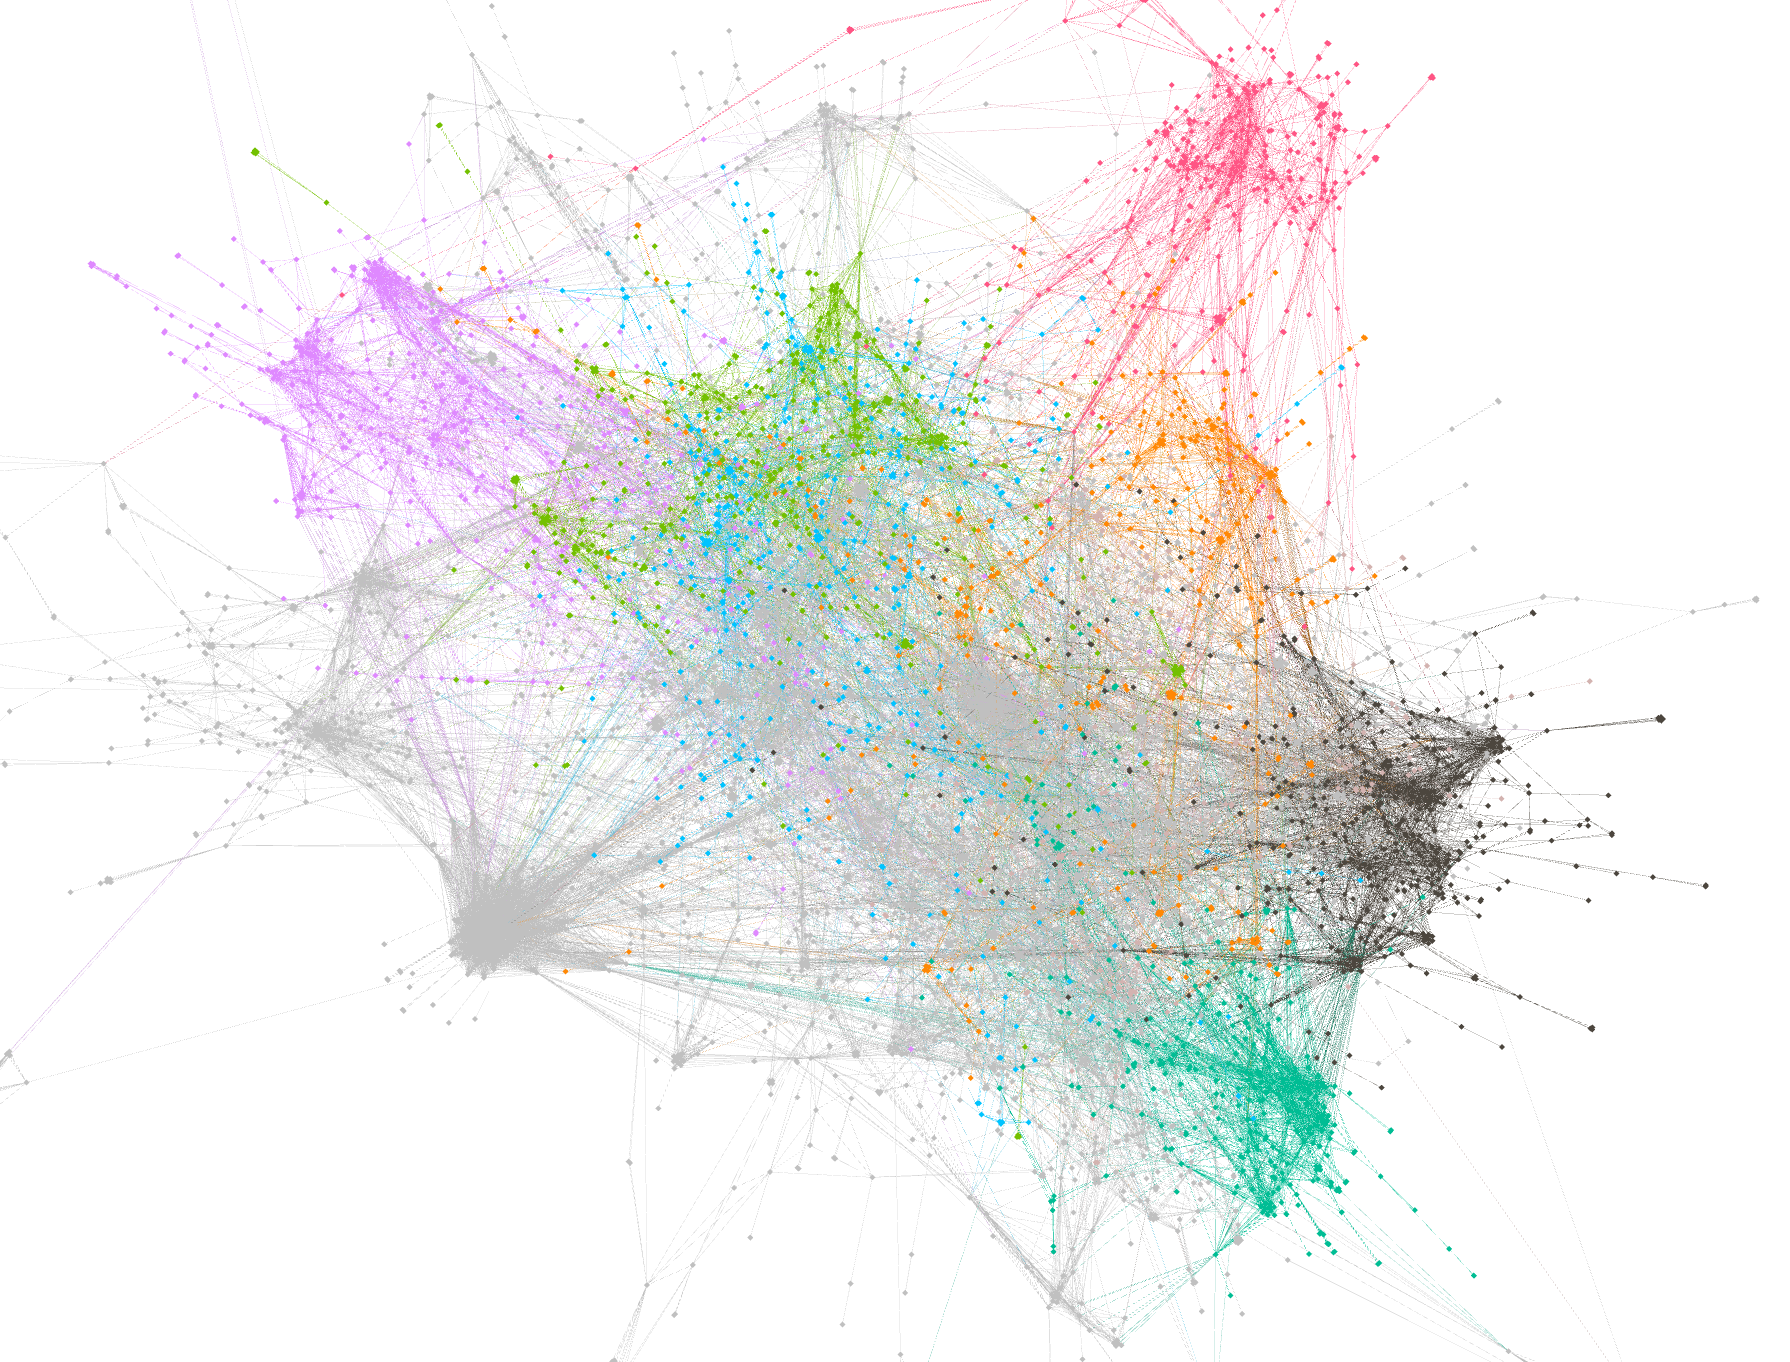
\includegraphics[width=0.23\textwidth]{imgs/one_day_net.png}
%     \caption{Contact network after one day}
%     \label{fig:my_label}
% \end{figure}

\begin{figure}
    \centering
    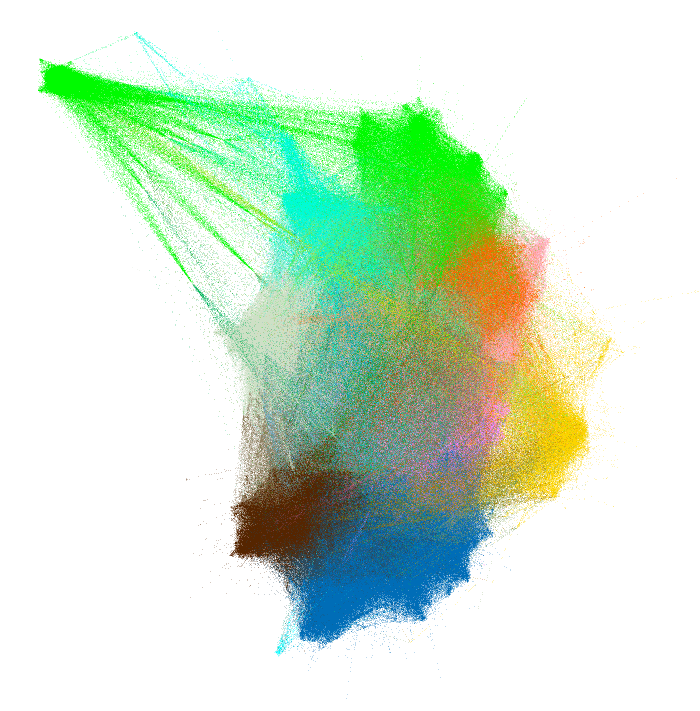
\includegraphics[width=0.23\textwidth]{imgs/5_day_network.png.png}
    \caption{5-Day Contact Network from July 1st, 2020 to July 5th, 2020}
    \label{fig:my_label}
\end{figure}

In Figure \ref{fig:my_label}, we can see the 5-Day Contact Network.
Network properties for this network were also calculated. The average node degree is 4.278, the network diameter is 20, the average clustering coefficient is 0.432, and the average path length is 6.95. In addition to this, the degree distribution was mainly an exponential distribution with subtle hints at a power-law. This can also be seen from the network itself, as we can see the presence of a few hubs in the network. This makes sense, as we should expect a social network to be scale-free, but we do not have all the data points, so it is not fully scale-free on the sample network.

In addition, we can see the resulting infected graph from our simulation in Figure \ref{fig:my_label2}.
\begin{figure}
    \centering
    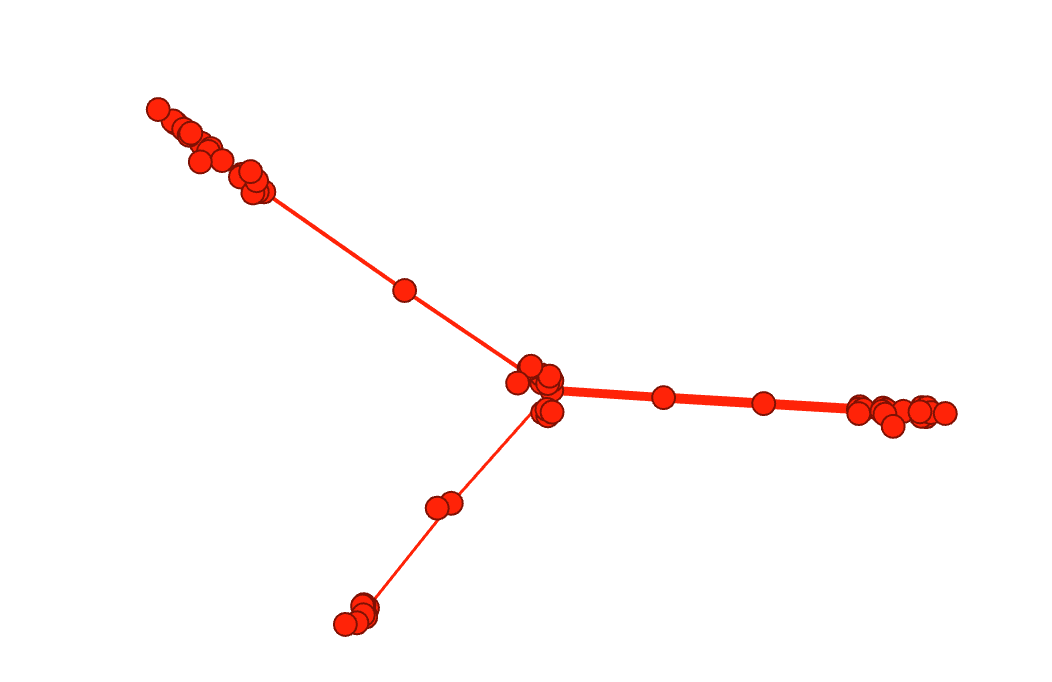
\includegraphics[width=0.23\textwidth]{imgs/simulation.png}
    \caption{Infected graph after one day}
    \label{fig:my_label2}
\end{figure}
In this network, it is important to note that all of the visible nodes are infected, and the edges represent how the infection has been spread. We can see that not a lot of infected nodes have spread the virus, but the ones that have created one connected component that show the beginnings of a scale-free network. 

In Figure \ref{fig:my_label3}, we can see the number of infected nodes over time. We can see that the infection doesn't spread much until the latter half of the day, after which it spreads steadily. We expect the rate of spread to be exponential when we simulate the spread over more days. This lines up with our intuition, as we would expect the infection to spread faster as more people get infected.
\begin{figure}
    \centering
    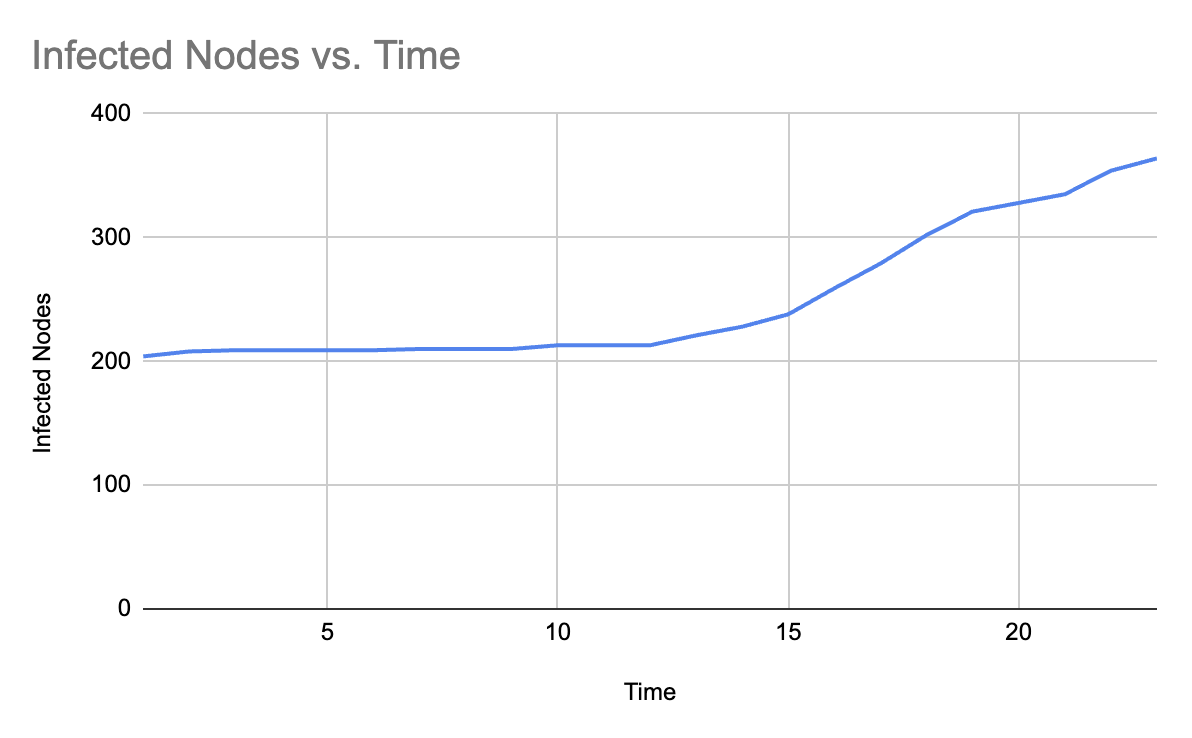
\includegraphics[width=0.28\textwidth]{imgs/infected_over_time.png}
    \caption{Number of infected nodes over 24 hours}
    \label{fig:my_label3}
\end{figure}


\Section{Conclusion and Short-Term Plans}
Through the analysis of the network, we were able to determine the network of contacts is a combination of an exponential and scale-free network. Some people came into contact with many other people whereas others stayed within their cliques. The simulation showed that the number of infected people initially stayed relatively constant, but after 12 hours, infections began increasing steadily.

For M2, we plan to do a more complete analysis of the network by considering both July and August data. We also plan to run more realistic simulations by accounting for the incubation period and deceased/recovered people. We also plan to implement GNNs at a small scale to perform link prediction. Specifically, we will use GNNs to predict the people that come into contact with previously infected people, allowing us to predict the spread of the virus.

% For this milestone, Afnan generated and analyzed the contact network and Jay created and analyzed the infection spread simulation.

For this milestone, Afnan generated and analyzed the contact network for July 1st, 2020, and Jaykumar created and analyzed the simulation of the hourly spread of the virus.


% For M2, we plan to do a more complete analysis of the network by considering both July and August data. We also plan to run more realistic simulations by accounting for the incubation period, deceased people, and recovered people. We also plan to implement GNNs at a small scale to perform link prediction. Specifically, we will use GNNs to predict the people that come into contact with previously infected people. By predicting contact between people, we will be able to predict the spread of the virus.

%------------------------------------------------------------------------- 
% \Section{Objectives and Deliverables}

% First, we will analyze the networks to determine their properties. Then, to better understand network behavior, we will run simulation to see how COVID-19 spreads through the network.

% The main goal of contact tracing is to find people who may be infected due to their contact with other infected people. Similarly, this project will aim to classify infected nodes in a graph, where nodes represent people, and links represent contact between people. This network will be formed by utilizing real contact information from mobile devices. In order to predict infections within a network, this project will implement and analyze GNNs, specifically link prediction. 

% The dataset we will be using is the ``foursquare'' mobility dataset that consists of location visit logs in Austin, TX from 2019 to 2021. The visit log includes information about when and where a device was, as well as how long it was there. 
% - What are the main research questions you plan to address?
% - How exactly is the “network” formed? What is a “node” and what is a “link”?
% - Which dataset(s) do you plan to use?
% - What are the deliverables?

%------------------------------------------------------------------------- 
% \Section{Tasks and Timeline}

% Firstly, we will collect and clean the data. This includes reformatting and filtering the data. We will analyze the dataset to get a better understanding of its properties (such as degree, betweenness centrality, clustering coefficient, etc.). We plan to complete this by October 10th, 2023.

% Then we plan to run simulations on the network to get a better understand of how the virus flows. We plan to complete this by November 14th, 2023.

% Finally, we will utilize GNNs to perform link prediction to see how the network evolves over time. We plan to complete this by November 30th, 2023.

% We will pair program; thus, the member contribution will be 50/50.

% - What are the main tasks of your project?
% - What is the proposed timeline (w.r.t. project milestones) and member(s) contribution?

%------------------------------------------------------------------------- 

% \Section{Conclusion and References}

% In conclusion, the project aims to utilize GNNs to make contact tracing more efficient and accurate. We will analyze the dataset to understand its properties, we will run simulations to see how the virus spreads through the network, and we will train GNNs to perform link prediction.

% We will start by researching GNNs. Particularly, we will look at an article by Neptune.ai on the application of GNNs and a DGL tutorial on link prediction \cite{menzli-blog} \cite{dglLinkPrediction}.

% https://towardsdatascience.com/graph-convolutional-networks-introduction-to-gnns-24b3f60d6c95
% https://neptune.ai/blog/graph-neural-network-and-some-of-gnn-applications#:~:text=Graph%20Neural%20Networks%20(GNNs)%20are,and%20graph%2Dlevel%20prediction%20tasks.
% https://docs.dgl.ai/en/0.8.x/tutorials/blitz/4_link_predict.html

% what a GNNs is, and how to use it (blogs on this).

% - Briefly summarize the project idea and main contributions.
% - Include some starting points (e.g., papers, websites, datasets, etc., preferably more than what
% was given to you as a starting point in the projects description).


%------------------------------------------------------------------------- 
% \nocite{ex1,ex2}
\bibliographystyle{latex8}
\bibliography{latex8}

\end{document}

